\section{Study of systematics on ringdown measurements \ab{in real , non-Gaussian noise}}\label{sec:noise_systematics}

\comment{AB: Please improve considerably this Appendix because it is not easy to follow the motivation and the logic. It is written for LIGO people.
I have tried to make changes but it is better if you do it. I risk to erase parts that you would consider important. Please write it thinking that your
reader is not an LSC reader!}

In Sec.~\ref{sec:method}, we \ab{discussed} \sout{mentioned that} the expression of the
Bayesian likelihood function \ab{that we use in our analysis} \sout{outlined in} \ab{(see
Eq.~\ref{eq:likelihood})} \ab{and stressed that it}\sout{and \ref{eq:nwip}} is only valid if the interferometric noise can be
described as a stationary Gaussian process. LIGO-Virgo noise, however,
frequently has non-stationary and/or non-Gaussian features, for
example glitches, which can affect parameter inferences unless
appropriately accounted for. Here we demonstrate\ab{, by injecting in real
noise a GW190521-like signal} \sout{with an example of a
GW190521-like simulated signal}, \ab{how} systematic biases \ab{can originate} \sout{likely originating}
from an incomplete understanding of the noise. \comment{AB: It is confusing to refer to ``systematic''
biases for the noise, generally we refer to systematic biases for the waveform modeling.
In fact, below you also, somewhat suddenly, refer to (lack of) precession, as a possible source of systemtcis.
I would advice you to clarify from the beginning of this Appendix, what this study is about and what you intend to
do below.}

%%%%%%%%%%%%%%%%%%%%%%%%%%%%%%%%%%%%%%%%%%%%%%%%%%%%%%%%%%%%%%%
%%%%%%%%%%%%%%%%%%%%%%%%%%%%%%%%%%%%%%%%%%%%%%%%%%%%%%%%%%%%%%%
\begin{figure}
\begin{center}
        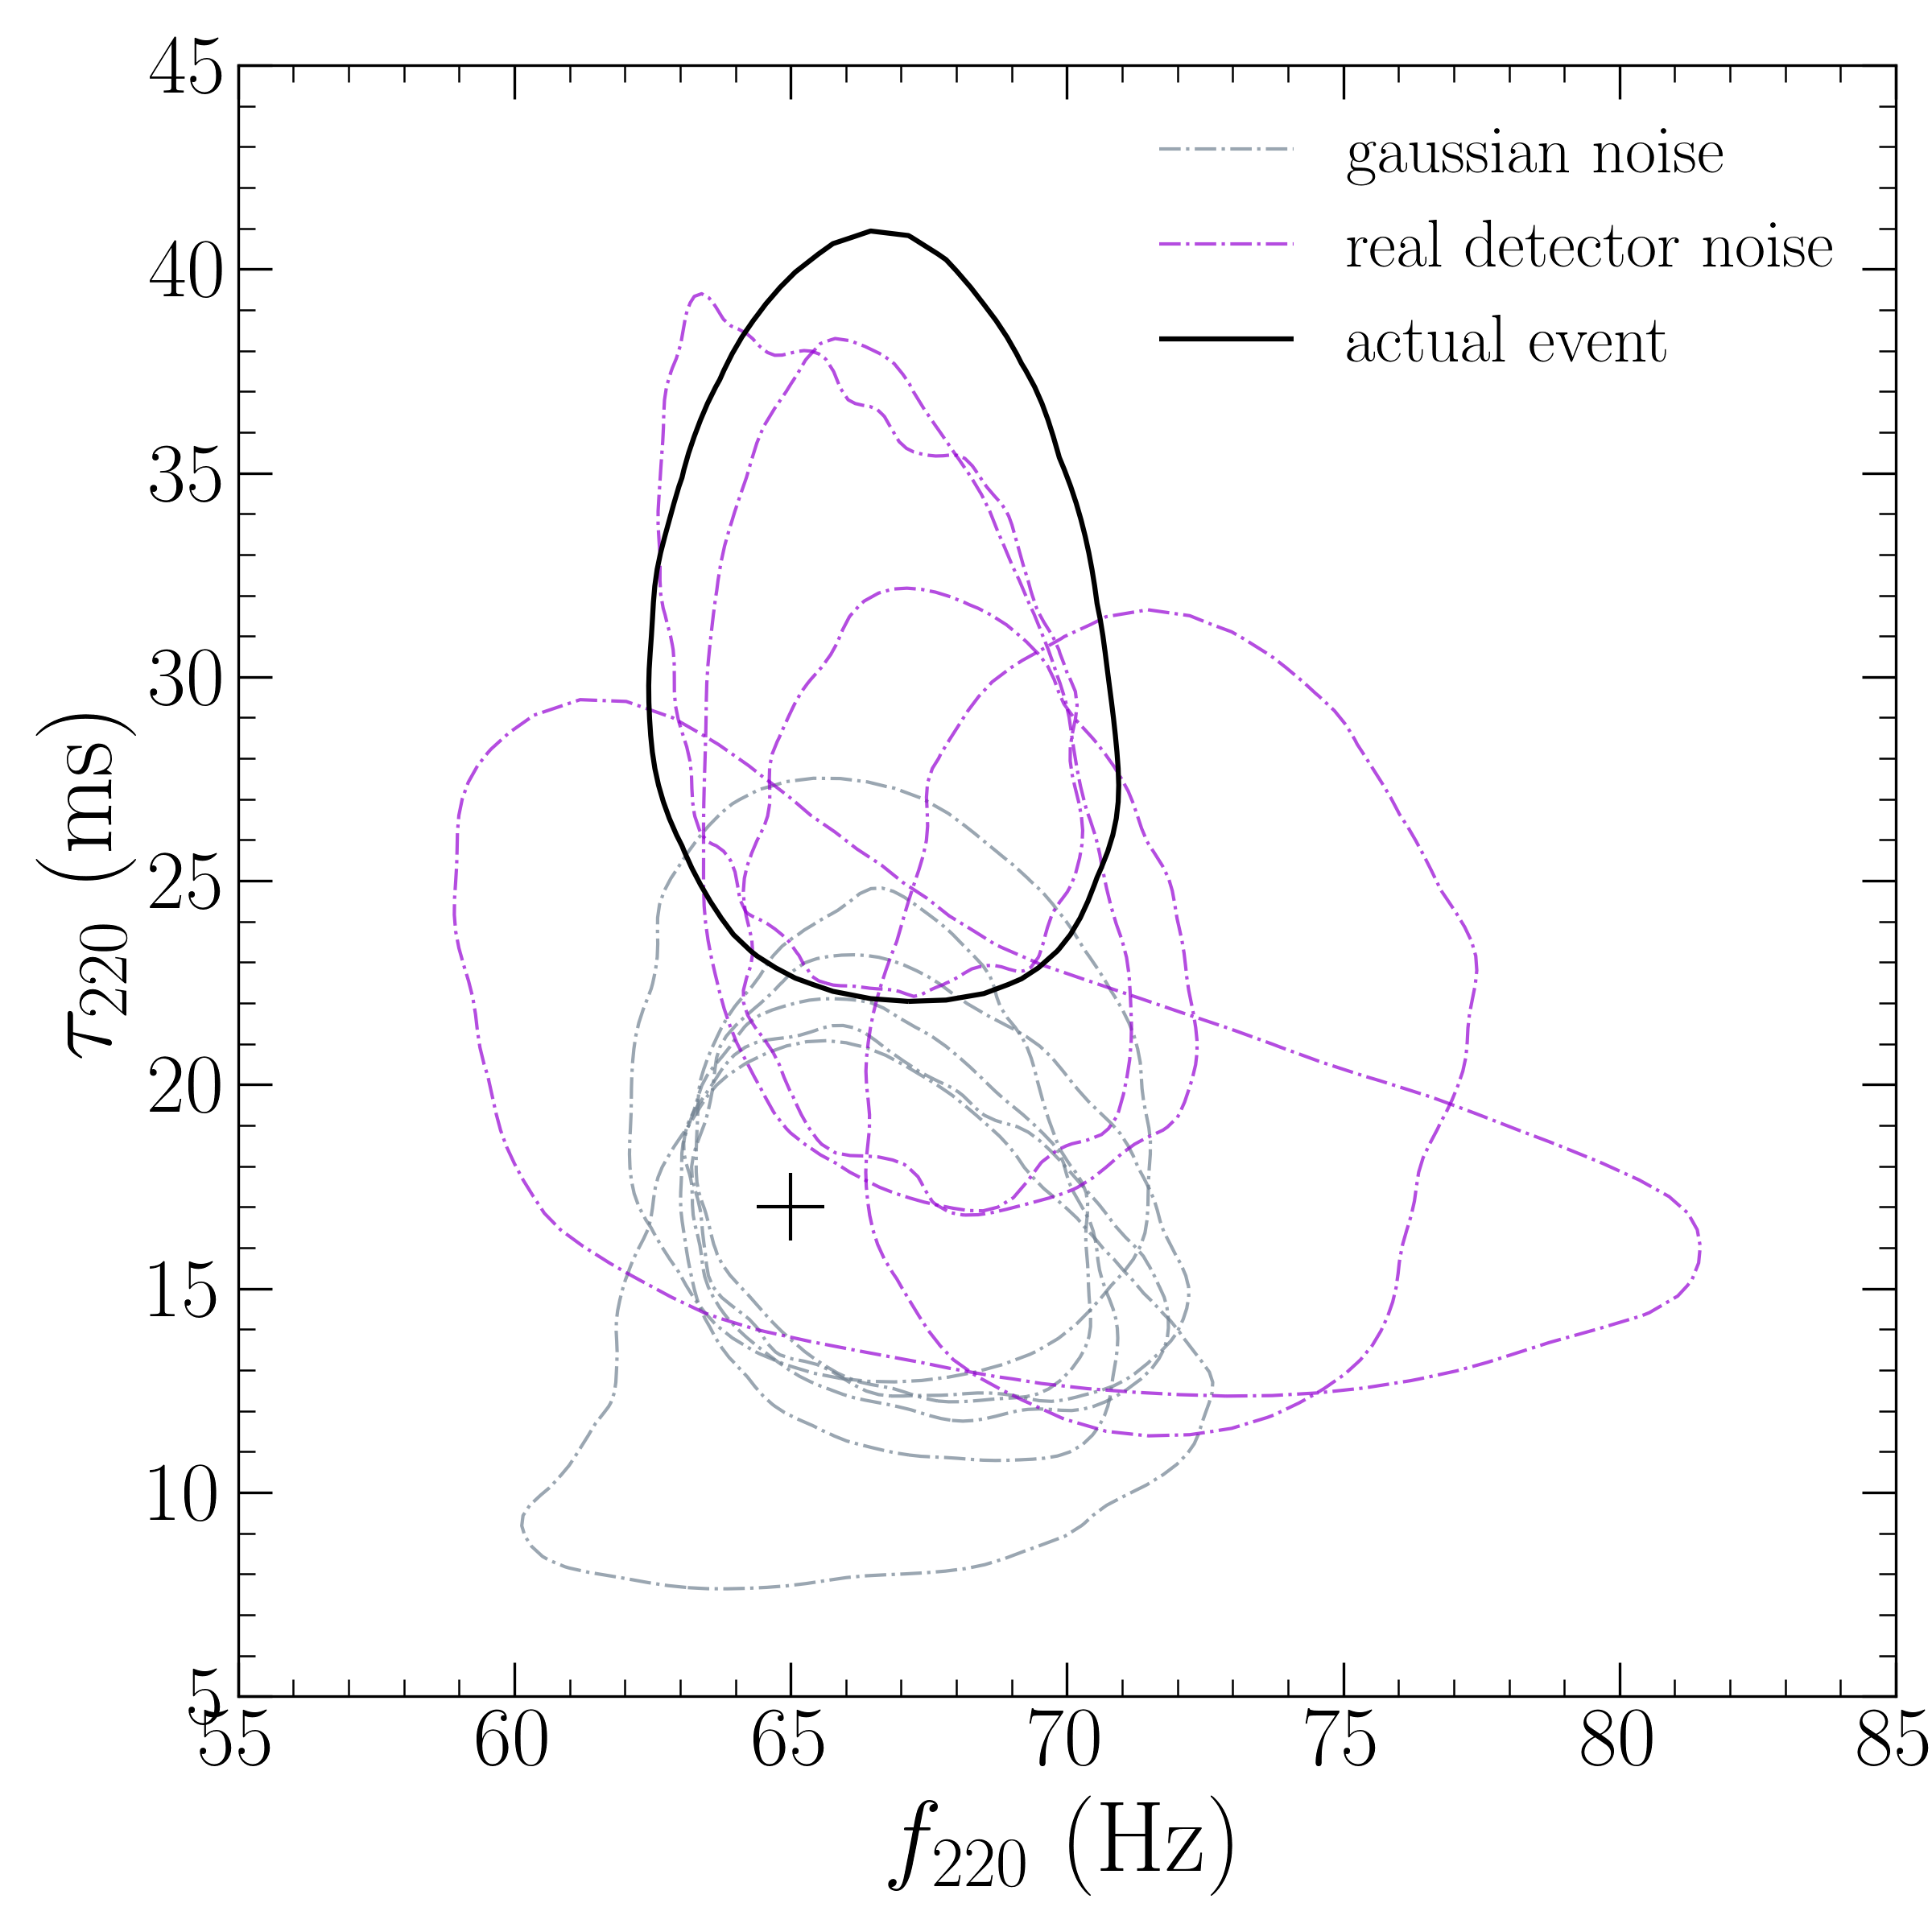
\includegraphics[width=0.5\textwidth]{figures/S190521g_swinjs.png}
        \caption{\textcolor{red}{FINAL RESULT} 90 \% credible level on the posterior probability distribution of the frequency and damping time of $(2,\pm 2)$ mode, $(\fgr{220}, \taugr{220})$ from simulations \comment{AB: I have changed this in other places. The word ``simulations'' is confusing, because we deal with a paper in which we also refer to NR simulations. I suggest to use ``injected synthetic signals'' instead} of an \texttt{NRSur7dq4} GW signal with parameters similar to the GW event, GW190521, in Gaussian noise (grey dot-dashed lines) and real interferometric noise (pink dot dashed lines). The GR prediction for the frequency and damping time is indicated by the black cross. While the Gaussian noise simulations are consistent with the prediction, at least 3 or the 5 real noise simulation are not. For comparison, we also plot the 90 \% credible level for the actual event, GW190521. \comment{AB: For clarity, please indicate on the plot which waveform model is used to obtain such posteriors, as you did
in the other plots of the paper. Also, please use something else instead of ``actual event'', which is confusing. The problem is
that the first two entries of the legend refer to the noise properties of the PE study done with an injected synthetic signal, whereas I believe ``actual event'' refers to ``real'' not injected signal
and ``real noise''. All the entries in the legend need to be consistent with each other; you need to specify for each of them the ``signal'' and the ``noise''. I hope is clear what I am saying}}
        \label{fig:21g_systematics}
\end{center}
\end{figure}
%%%%%%%%%%%%%%%%%%%%%%%%%%%%%%%%%%%%%%%%%%%%%%%%%%%%%%%%%%%%%%%
%%%%%%%%%%%%%%%%%%%%%%%%%%%%%%%%%%%%%%%%%%%%%%%%%%%%%%%%%%%%%%%

\ab{The spinning, precessing NR-surrogate model \texttt{NRSur7dq4}, valid up to mass ratio 4, was employed
(together with the $\SEOB$ model) to analyze the GW190521 signal observed by the LIGO and Virgo detectors.
For the injected synthetic signal we use a \texttt{NRSur7dq4} waveform with parameters similar to the ones
recovered by this model on the actual GW190521 data (see Table I of Ref.~\cite{Abbott:2020tfl}).}
\ab{In Fig.~\ref{fig:21g_systematics}, we indicate with a black cross what the injected \texttt{NRSur7dq4} signal
predicts for the $(2,2)$ frequency and damping time, and for comparison, we also
show with a black solid curve the results obtained when recovering the the actual signal GW190521 with the waveform model $\pSEOB$. As seen in the plot, while
the measurement of the frequency is consistent with the prediction, we overestimate the damping time.} \comment{AB: it is not clear
to me what the figure shows. Is the black line the result when running $\pSEOB$ against real data or the
injection in realt data?}

\comment{AB: What is the ``underlying'' NR signal? I think you are referring to the
injected signal. Also, until now you have not discussed precession.
} The underlying NR signal is expected to be precessing, and since the
$\pSEOB$ model is built on an aligned-spin GR model, a lack of
precession could bias measurements. We explore effects of possible
waveform systematics by injecting the signal is coloured Gaussian
noise. In this case, since the understanding of the noise realizations
is complete, any measurement biases could only arise from incomplete
understanding of the \sout{underlying} \ab{injected} signal. We find (grey curves in
Fig.\ref{fig:21g_systematics}) our results to be consistent with the
prediction thus ruling out a lack of precession to be a likely cause
for the bias in the damping time measurement of the actual signal.

We subsequently study the effects of possible noise systematics by
injecting the same \texttt{NRSur7dq4} GW signal in different
realizations of actual interferometric noise around the real event
GW190521. Since the PSDs of the GW detectors are expected to vary over
longer durations of time, we select 5 different noise realizations
over a segment of 2.5 hours of coincident data in both the LIGO
detectors centered at the time of the actual event. The noise
properties in this chunk of data, and consequently for all 5 simulated
signals, is expected to be the closest to that for the actual
event. The results are indicated by \sout{pink} \ab{green} curves in
Fig.~\ref{fig:21g_systematics}. \ab{As it can be seen from the figure,}
for 3 of the 5 noise realizations,
corresponding to $t_0-1$ hour, $t_0+0.5$ hours, and $t_0+1$ hour we
recover a damping time similar to the actual event, where $t_0$ is the
GPS time of the actual event. For the other two noise realizations, we
estimate the consistent damping time but an off-set frequency, while
the fifth noise realization is consistent with both predictions. The
SNR in the Livingston detector goes down by more than \ab{a factor} 3 in some
runs, indicative of how a variation in the noise strongly affects our
ability to infer parameters. This also seems to indicate that a bias
in the measurements of the damping time for the actual event \comment{AB: not clear
what you mean} can be unaccounted noise systematics.

